%%%%%%%%%%%%%%%%%%%%%%%%%%%%%%%%%%%%%%%%%%%%%%%%%%%%%%%%%%%%%%%
\section{Photon Detector Efficiency Simulation}
\label{sec:fdsp-pd-simphys}
%\metainfo{(Length: \dword{tdr}=50 pages, TP=20 pages)}
%\metainfo{\color{blue} Content: Conveners}
% Provided by Alex H. 15mar18

The potential physics performance of \dword{pd} designs will be evaluated using a full simulation, reconstruction, and analysis chain developed for the \larsoft framework. The goal is to evaluate the performance in physics deliverables for each of the photon collector designs under consideration. The metrics evaluated will include efficiency for determining the time of the event ($t_0$), timing resolution, and calorimetric energy resolution for three physics samples: \dword{snb} neutrinos, nucleon decay events\footnote{The most relevant sample is actually the \emph{background} to nucleon decay events. However, efficiently simulating background that can mimic nucleon decays is challenging since they can be quite rare topologies, so it is easier to simulate the nucleon decay signal which should be representative of the background.}, and beam neutrinos. However, the development of analysis tools to take advantage of this full simulation chain is fairly recent, so this proposal will only include one test case: $t_0$-finding efficiency for \dword{snb} neutrinos versus the effective area of the photon collectors (see Section~\ref{sssec:photoncollectors}).

The first step in the simulation specific to the \dword{pds} is the simulation of the production of light and its transport within the volume to the \dwords{pd}. Argon is a strong scintillator, producing \SI{24000}{$\gamma$s/MeV} at our nominal drift field. Even accounting for the efficiency of the \dwords{pd}, it is prohibitive to simulate every optical photon with \dword{geant4} in every event. So, prior to the full event simulation, the detector volume is voxelized and many photons are produced in each voxel. The fraction of photons from each voxel reaching each photosensor is called the \textit{visibility}, and these visibilities are recorded in a 4-dimensional library (akin to the \textit{photon maps} used in the \dword{dpmod} simulation (see \voltitledpfd~Section 6.1.1).
% described in Section~\ref{subsec:fddp-pd-6.1.1}). 
% doesn't appear possible to reference a section in the other volume.
This library includes Rayleigh scattering ($\lambda=$ \SI{55}{cm}\cite{Grace:2015yta}), absorption ($\lambda=$ \SI{20}{m}), and the measured collection efficiency versus position of the double-shift light-guide bars. When a particle is simulated, at each step it produces charge and light. The light produced is distributed onto the various \dwords{pd} using the photon library as a look-up table and the early (\SI{6}{ns}) plus late (\SI{1.6}{$\mu$s}) scintillation time constants are applied. Transport time of the light through the \lar is not currently simulated, but is under development.

The second step is the simulation of the electronics response. For now, the \dword{sipm} signal processor (\dword{ssp}) readout electronics used for \dword{pd} development and in \dword{pdsp} is assumed (see Section~\ref{sec:fdsp-pd-pde}). 
Waveforms are produced on each channel by adding an \dword{sipm} single-\phel response shape for each true photon. In addition, other characteristics of the \dword{sipm} are included such as dark noise, crosstalk and afterpulsing, based on data from device measurements. 
%) From Alex 4/17/18 - We do include afterpulsing as well, at rates based on the sensl sipm's tested in Hawaii. You can just add it to the list of things included in the electronics simulation. 
Dark noise, at a rate of \SI{10}{Hz} for each of the three \dword{sipm}s on each channel is include by the addition of extra single-\phel waveforms. Crosstalk (where a second cell avalanches when a neighbor is struck by a photon generated internal to the silicon) is introduced by adding a second \phel \num{16.5}\% of the time when an initial \phel is added to the waveform. Additional uncorrelated random noise is added to the waveform with an RMS of \SI{2.6}{ADC} (or approximately \SI{0.1}{\phel}). The response of the SSP self-triggering algorithm, based on a leading-edge discriminator, is then simulated to determine if and when a \SI{7.8}{$\mu$s} waveform will be read out, or in the case of the simulation it will be stored and passed on for later processing.

The third step is reconstruction, which proceeds in three stages. The first is a ``hit finding'' algorithm that searches for peaks on individual waveforms channel-by-channel, identifying the time based on the time of the first peak and the total amount of light collected based on the integral until the hit goes back below threshold. The second step is a ``flash finding'' algorithm that searches for coincident hits across multiple channels. All the coincident light is collected into a single object that has an associated time (the earliest hit), an amount of light (summed from all the hits), and a position on the plane of the \dwords{apa} ($y$-$z$) that is a weighted-average of the positions of the photon collectors with hits in the flash\footnote{Currently, the flash reconstruction does not consider the positions of the hits, only their times. 
This will need to be updated in the future when we simulate the full-sized \dword{spmod} but for now we are working in a small test geometry that acts as a crude simulation of this kind of constraint.}. The final step is to ``match'' the flash to the original event by taking the largest flash within the allowed drift time that is within \SI{240}{cm} in the $y$-$z$ plane. Since the TPC reconstruction is still in active development, especially for low-energy events, we match to the true \dword{mc} vertex of the event in the analyses presented here. This is a reasonable approximation since the position resolution of the TPC will be significantly better than that of the \dword{pds}. 

\begin{dunefigure}[Preliminary estimates of the efficiency for finding $t_0$ for SNB events.]{fig:pds-snefficiency}
{Preliminary estimates of the efficiency for finding $t_0$ for core collapse \dword{snb} events vs. the effective area (top), distance from the anode plane (bottom-left), and neutrino energy (bottom-right).}
  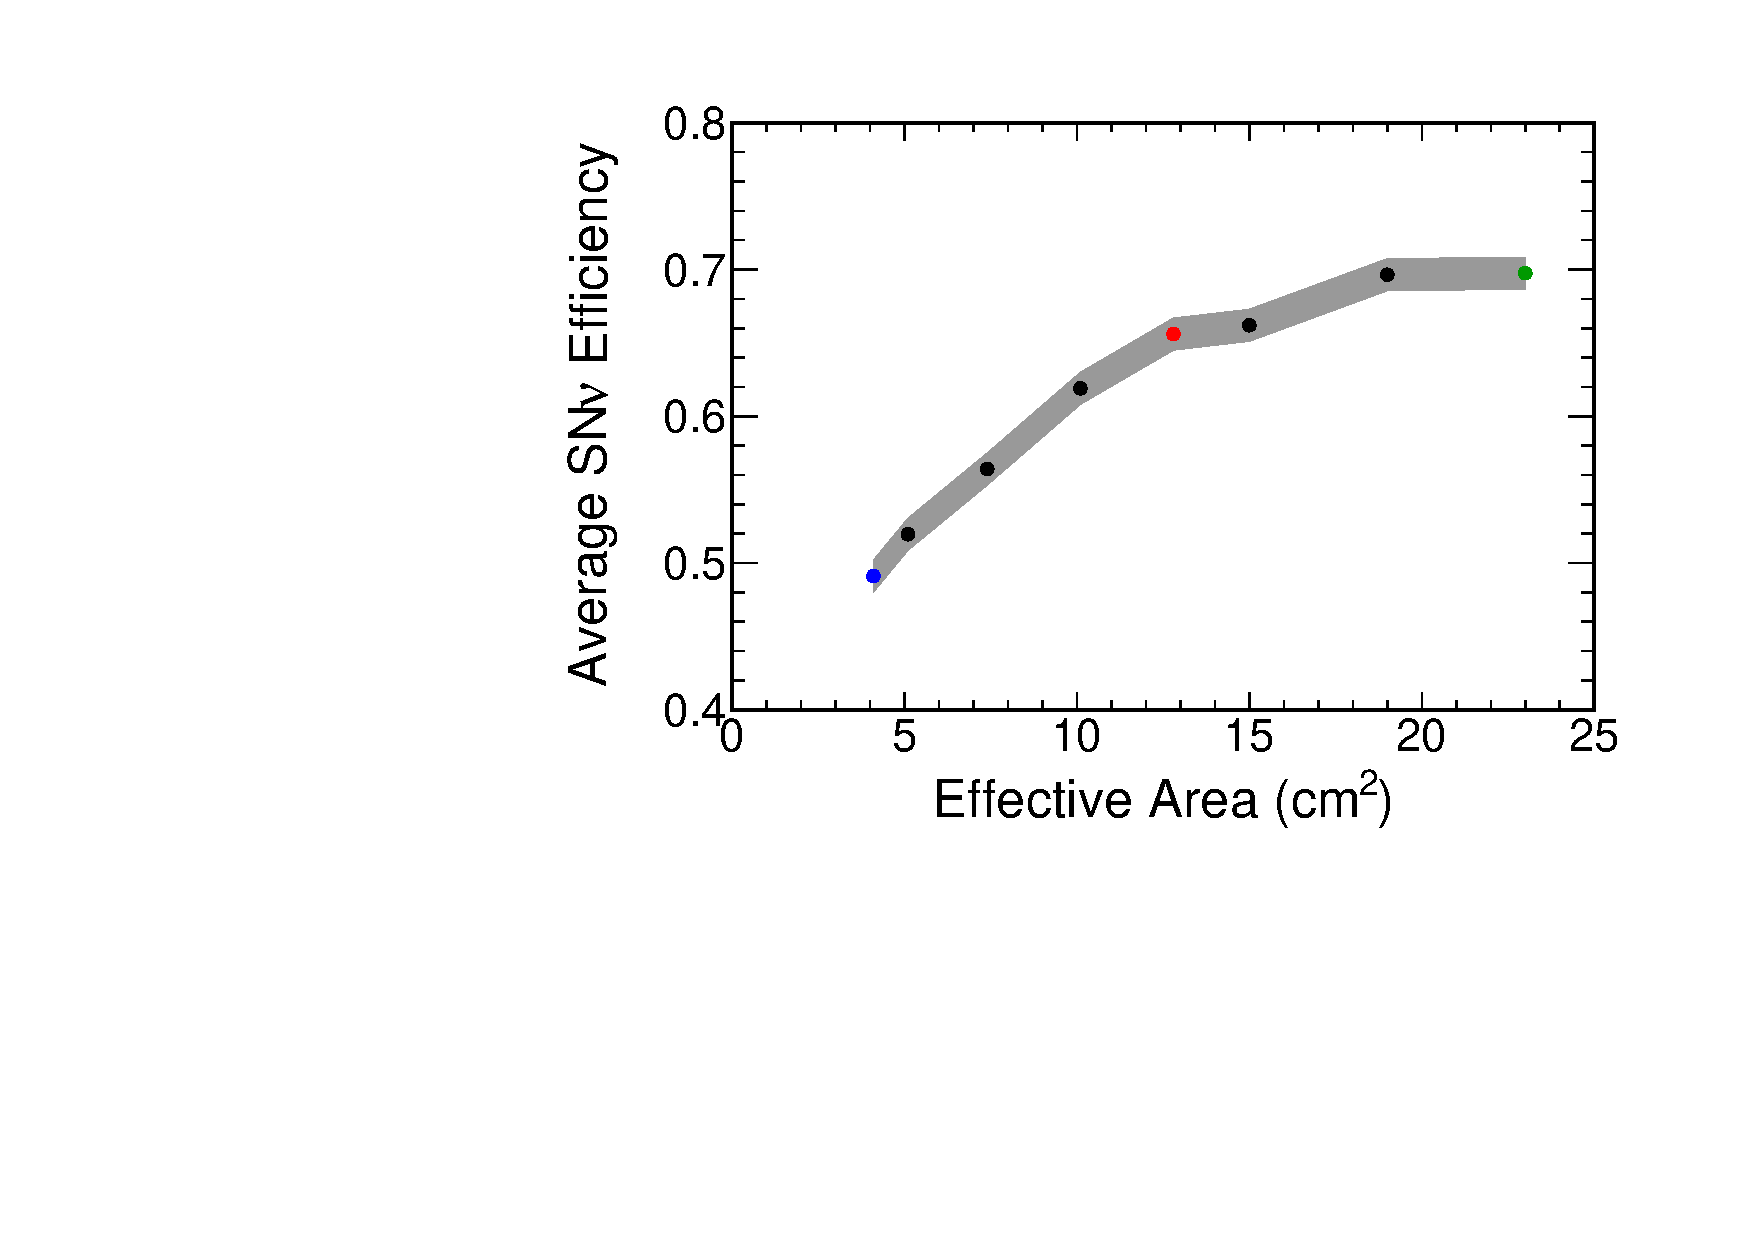
\includegraphics[width=0.4\columnwidth]{pds-efficiency.pdf}\\
%\end{dunefigure}
%\begin{dunefigure}[Efficiency for finding $t_0$ for supernova neutrino events vs. distance from the andode plane. NOTE: numbers are not final.]{fig:pds-sneff-x}
%{Efficiency for finding $t_0$ for supernova neutrino events vs. distance from the andode plane. NOTE: numbers are not final.}
  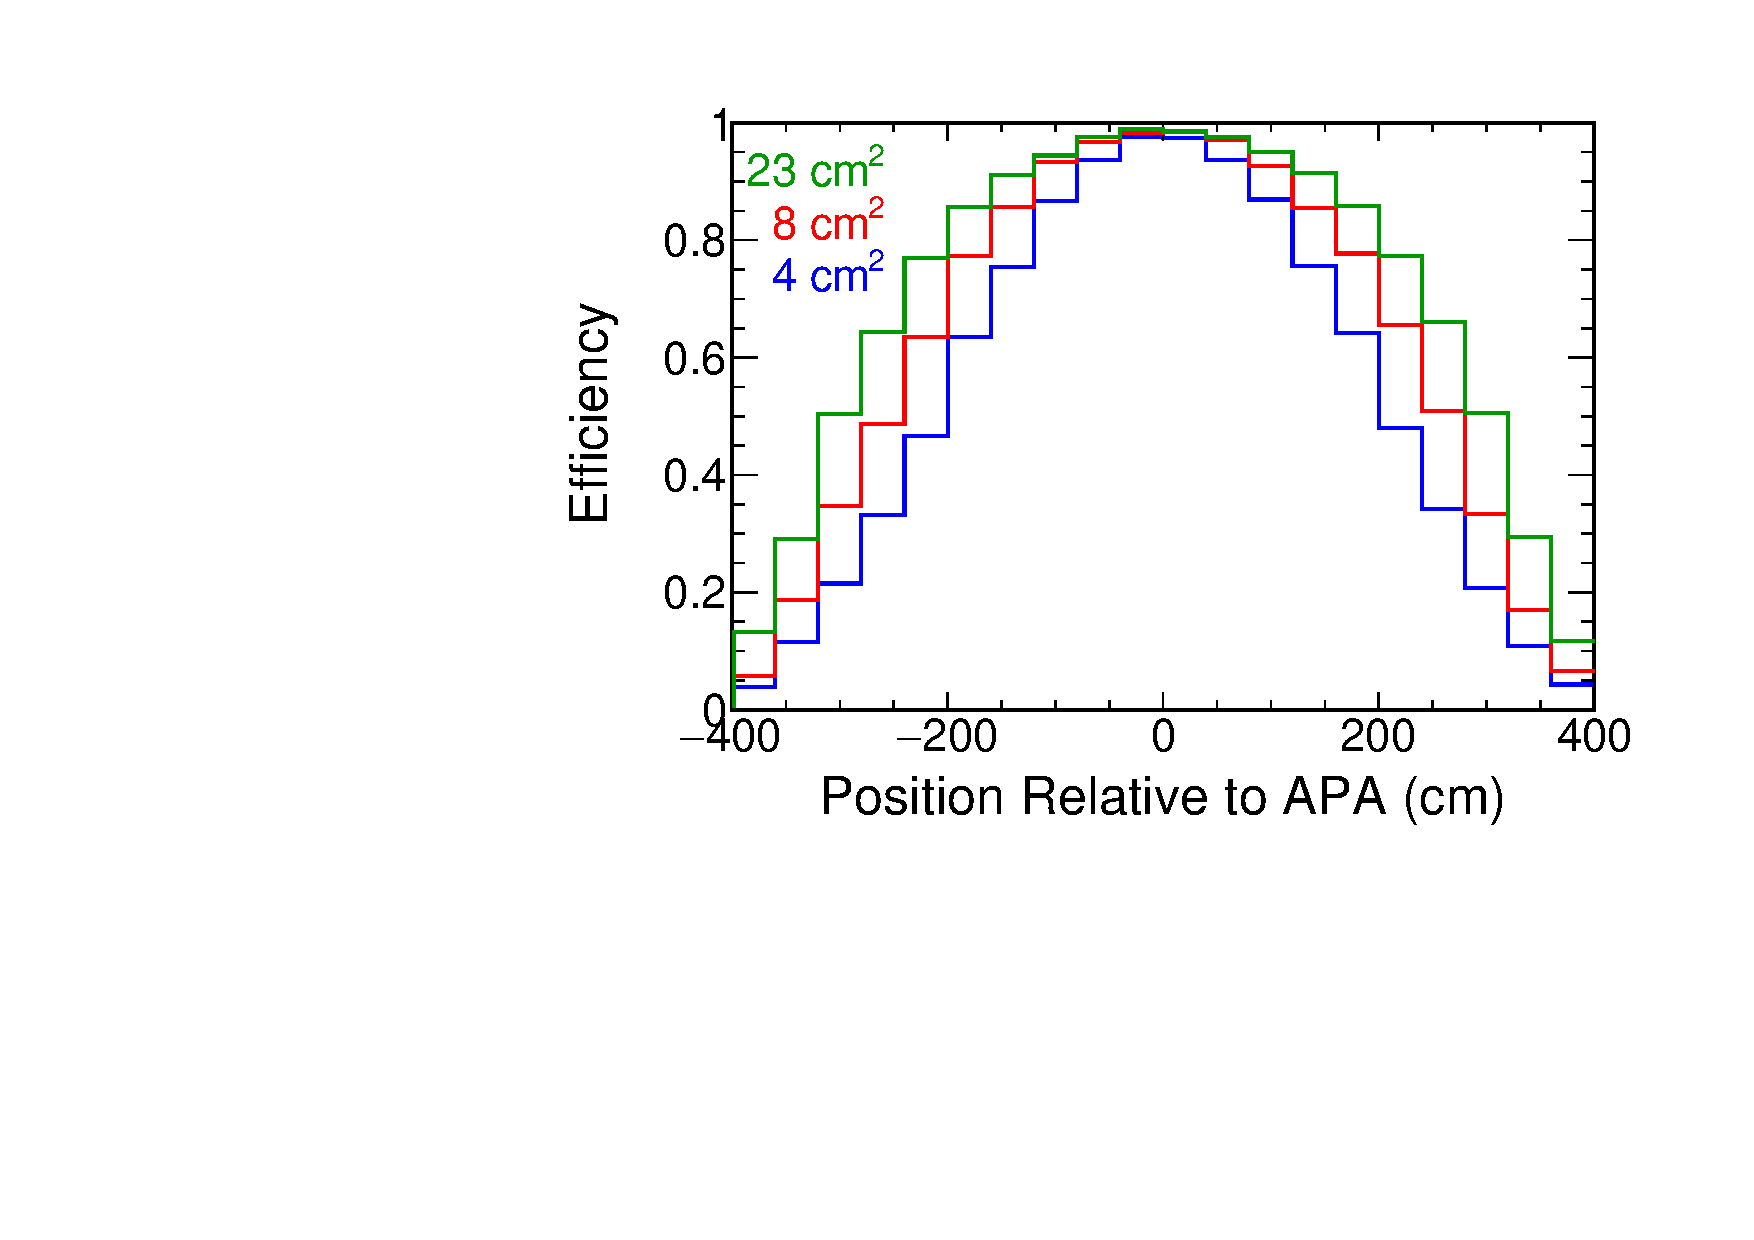
\includegraphics[width=0.4\columnwidth]{pds-position.pdf}
%\end{dunefigure}
%\begin{dunefigure}[Efficiency for finding $t_0$ for supernova neutrino events vs. neutrino energy. NOTE: numbers are not final.]{fig:pds-sneff-e}
%{Efficiency for finding $t_0$ for supernova neutrino events vs. neutrino energy. NOTE: numbers are not final.}
  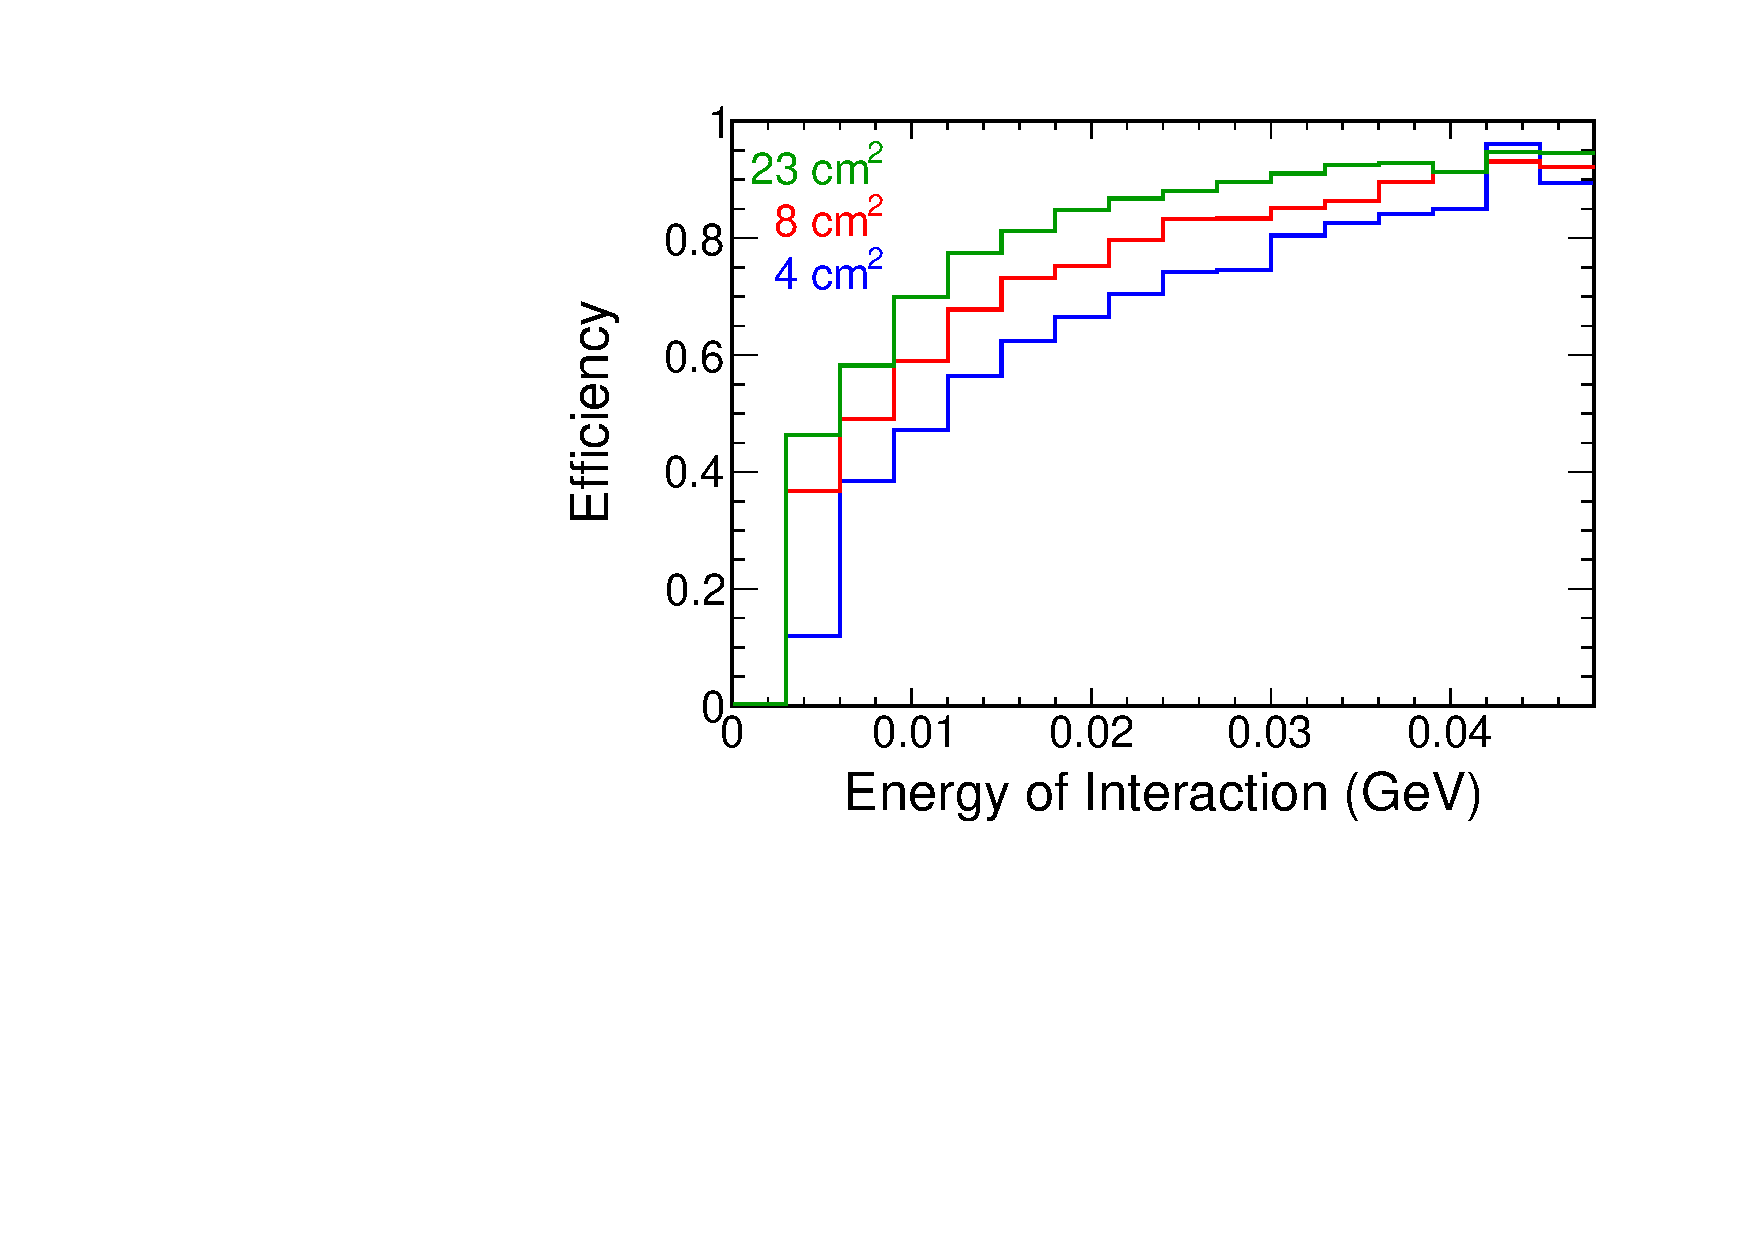
\includegraphics[width=0.4\columnwidth]{pds-energy.pdf}
\end{dunefigure}

%Figure~\ref{fig:pds-snefficiency}~(top) shows the efficiency for determining $t_0$ for events in a typical supernova spectrum using the tools above. The changes in effective areas that would correspond to alternative photon collection designs are achieved by simply scaling the total efficiency of the simulated double-shift light guide design shown here. The differences in attenuation behaviors within the bars are a second-order effect relative to the total amount of light collected. The efficiency for finding $t_0$ for these events increases linearly up through about \SI{15}{cm^2} of effective area, at which point the gains begin to slow down. Figures~\ref{fig:pds-snefficiency}~(bottom-left) and \ref{fig:pds-snefficiency}~(bottom-right) show how the efficiency varies as a function of neutrino energy and distance from the anode plane for three chosen points.

Figure~\ref{fig:pds-snefficiency}~(top) shows the efficiency for determiningt $t_0$ for events in a typical \dword{snb} spectrum using the tools above. The changes in effective areas that would correspond to alternative photon collection designs are achieved by simply scaling up the total efficiency of the simulated double-shift light guide design shown here. The differences in attenuation behaviors within the bars are a second-order effect relative to the total amount of light collected. The efficiency for finding $t_0$ for these events increases, but less than linearly as the performance of the light collectors is improved. Figures~\ref{fig:pds-snefficiency}~(bottom-left) and \ref{fig:pds-snefficiency}~(bottom-right) show how the efficiency varies as a function of neutrino energy and distance from the anode plane for three chosen points. Note that these algorithms are still in development so there is potential for improvement in the performance as development continues.

\begin{dunefigure}[Resolution on $t_0$ for \dword{snb} events.]{fig:pds-snt0}
{Resolution on $t_0$ for \dword{snb} events. These are based on simulation with effective light collector area of \SI{4}{cm^2}, which corresponds to the the photon detection efficiency of 0.23\% measured for a double-shift light guide module.}
%{Resolution on $t_0$ for supernova events. These are based on simulation with effective light collector area of \SI{4}{cm^2}.}
  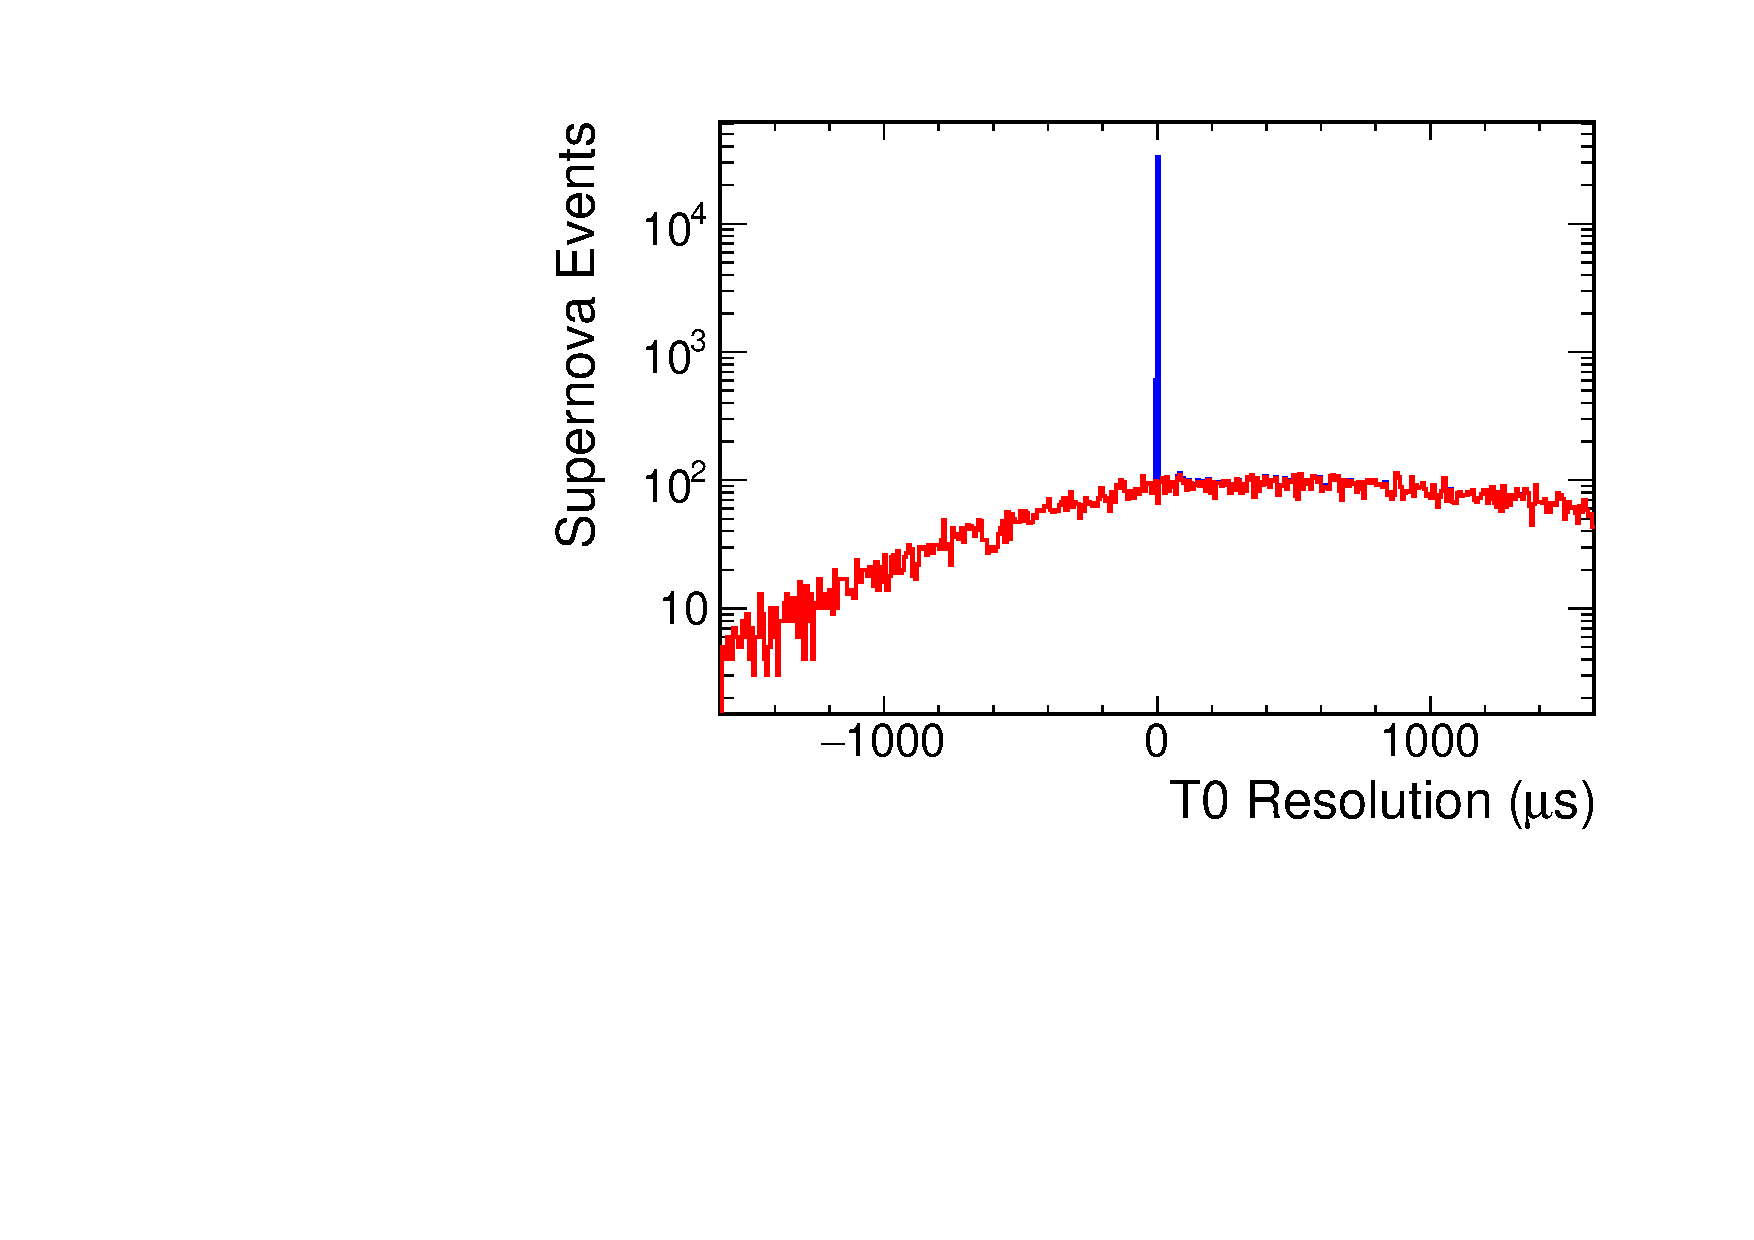
\includegraphics[width=0.4\columnwidth]{pds-t0res2.pdf}\\
  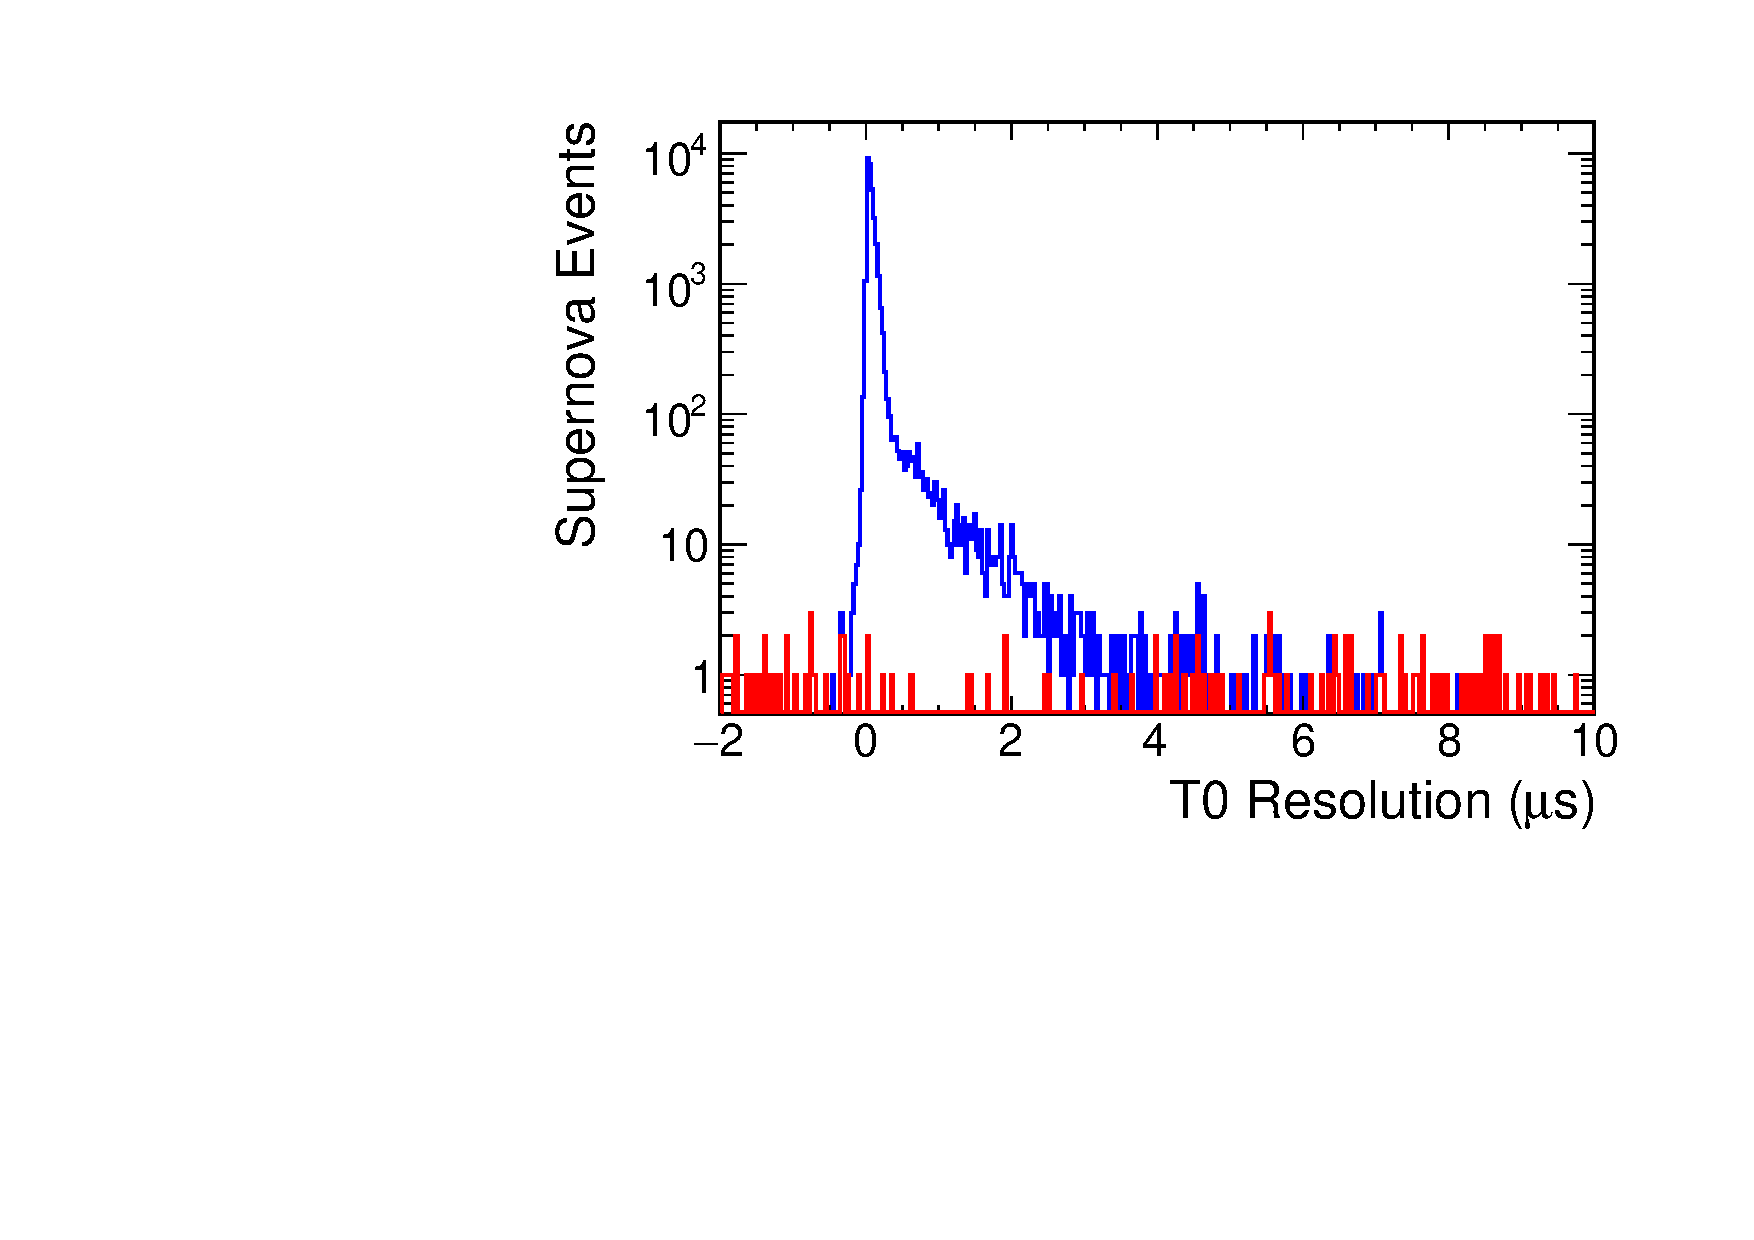
\includegraphics[width=0.4\columnwidth]{pds-t0reszoomed2.pdf}
\end{dunefigure}

If the correct flash is identified for a \dword{snb} event, the resolution on $t_0$ is excellent, as shown in Figure~\ref{fig:pds-snt0} -- for 95\% of the events, the time is identified from the prompt light and the timing resolution is better than \SI{100}{ns}, well within a single TPC time tick. In the remaining 5\% of cases where a correct flash is matched, the $t_0$ is biased towards later times (with respect to the true event time) by a few $\mu$s, driven by the late light time constant. If the wrong flash is identified the $t_0$ found is essentially randomly distributed in the drift time.

This preliminary study shows that each of the \dword{pd} options, with effective area per module currently estimated to be in the range  \numrange{4}{22}\si{cm$^2$}, will be able to determine the event $t_0$ with reasonable efficiency and it illustrates the benefit of higher photon detection efficiency. 

%%%%%%%%%%%%%% The following provided by Denver - superseded by the plots from Alex or incorporate into this section? %%%%%%%%%%%%%%%%%
%%
%Low-energy neutrinos from a galactic core-collapse supernova represent one of the most challenging physics channels for the photon detection system and Figure~\ref{fig:pds-sn-eff-simulation} shows the impact of improved \dword{pd} system performance on neutrino detection efficiency as a function of the energy of the electron produced in the neutrino interaction (this study was done for the double-shift light guide design).  The curve labeled ``standard'' corresponds to the current level of performance and results in an average efficiency for the photon detection system to unambiguously reconstruct the neutrino interaction time to be \num{30}\% at \SI{5}{MeV} and \num{70}\% at \SI{15}{MeV} of visible energy. A factor of two increase in \dword{pd} light yield increases the efficiency at \SI{5}{MeV} by almost \num{70}\%. 
%Validation of the simulations will come from extensive data from ProtoDUNE-SP and additional smaller scale prototypes underway or planned..

%\begin{dunefigure}[Neutrino detection efficiency dependence on \dword{pd} system performance.]
%{fig:pds-sn-eff-simulation}
%{Preliminary neutrino detection efficiency estimate as a function of the energy of the electron produced in the neutrino interaction for a variety of relative efficiencies of the double-shift light guide detector. The curve marked ``standard'' represents performance of recent prototypes.} 
%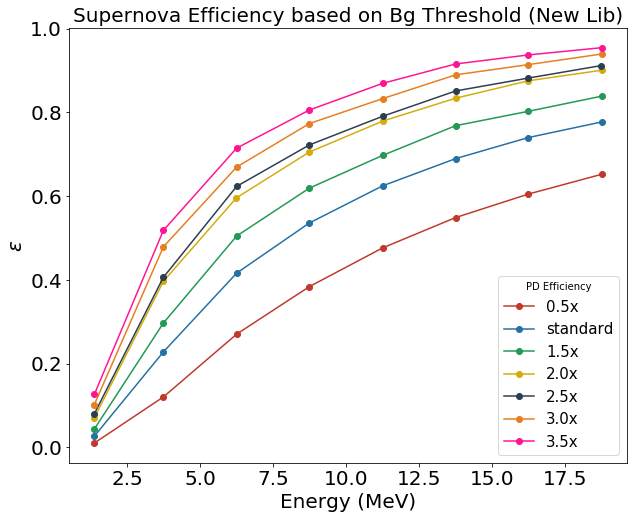
\includegraphics[width=0.5\columnwidth]{pds-sn-eff-simulation.png}
%\end{dunefigure}
%%
%%%%%%%%%%%%%%%%%%%%%%%%%%%%%%%%%%%%%%%%%%%%%%%%%%%%%%%%%%%%%%%%%%%%%%%%%%%%%%%%%%%%%%%%%%%
